\chapter{Thiết kế hệ thống}\label{chap2}
\section{Kiến trúc hệ thống}\label{sec:system-architecture}
Nền tảng hạ tầng của ứng dụng quản lý quán ăn được thiết kế giúp hướng đến tính ổn định cao và phát triển cho sau này.
Khi hệ thống đạt một số lượng người dùng nhất định, và có thể những người dùng này trải dài khắp nơi thay vì tập trung chủ yếu tại một địa điểm cố định.
Khi đó, việc duy trì một máy chủ vật lý sẽ không còn là lựa chọn tối ưu do sự tốn kém về nhân lực cũng như chi phí phát sinh trong việc bảo trì và nâng cấp cho máy chủ.
Từ đó mô hình kiến trúc của dự án hướng tới triển khai trên môi trường đám mây, tức sử dụng máy chủ của các nhà cung cấp dịch vụ đám mây rải rác ở khắp nơi trên thế giới.
Điều này sẽ giúp giảm đáng kể thời gian cấu hình máy chủ vật lý của hệ thống cũng như thời gian cần phải bỏ ra giúp duy trì và bảo dưỡng do các tác nhân bên ngoài gây nên.

\begin{figure}[h]
	\centering
	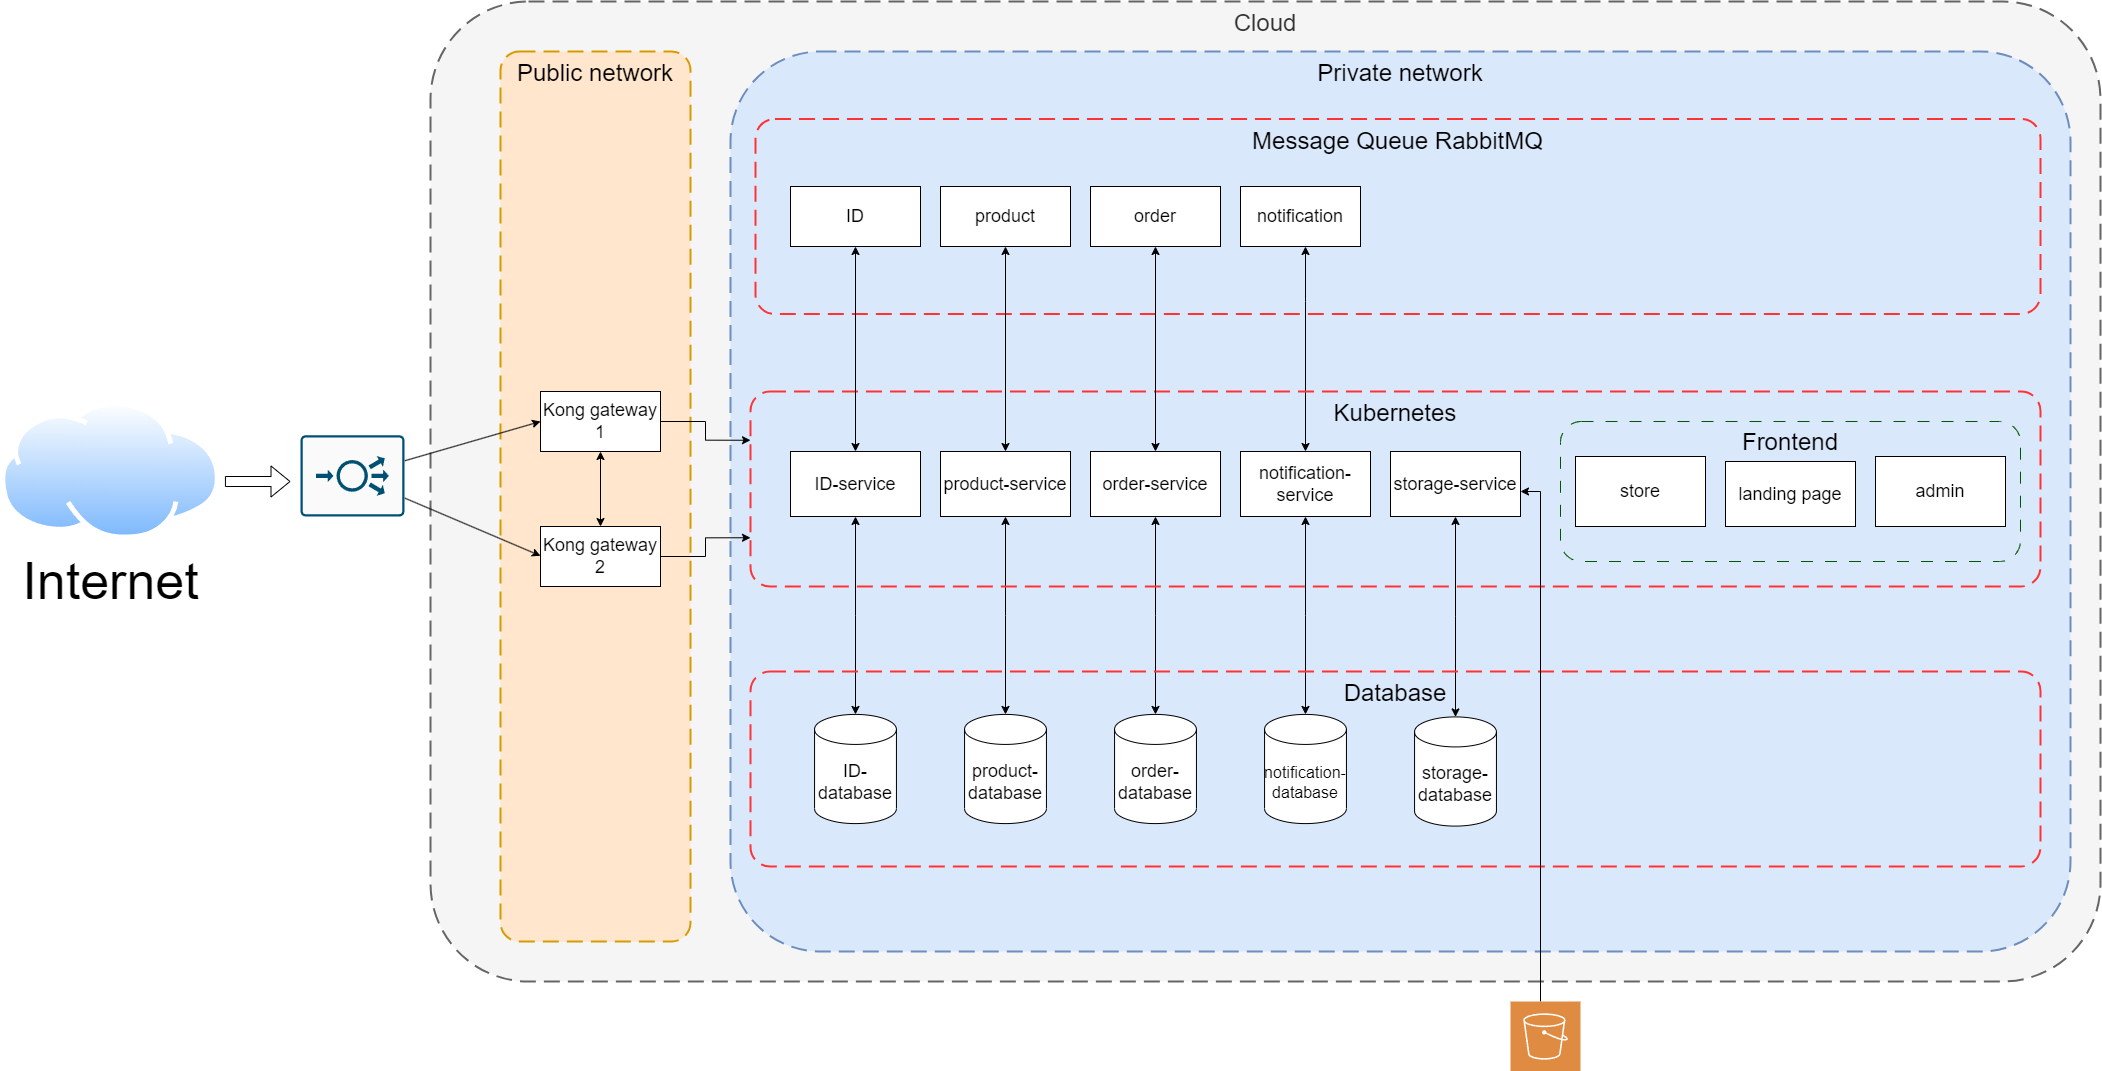
\includegraphics[width=1\textwidth]{images/hChip/overall-architecture.png}
	\caption{Kiến trúc tổng quan của hệ thống quản lý quán ăn}
	\label{fig:overall-architecture}
\end{figure}

Luồng dữ liệu đi vào hệ thống bắt nguồn từ ngoài Internet, nơi tất cả các yêu cầu của người dùng đi qua một GLSB (Global Server Load Balancers).
GSLB của Cloudflare giúp phân phối người dùng ở bất cứ nơi nào trên thế giới đến máy chủ khỏe mạnh gần nhất đối với họ.
Điều này sẽ giúp tối ưu hóa thời gian tải trang, giảm thiểu độ trễ, và đảm bảo trải nghiệm truy cập website của người dùng nhanh chóng, mượt mà nhất.
Ngoài ra Cloudflare còn đóng vai trò như một hệ thống phân giải tên miền (DNS).

Khi người dùng truy cập vào trang giới thiệu hoặc trang quản lý nhà hàng lần đầu tiên trên trình duyệt web, trình duyệt sẽ gửi truy vấn tới máy chủ DNS cục bộ (resolver), thông thường sẽ là máy chủ của nhà mạng.
Máy chủ DNS cục bộ sẽ kiểm tra liệu tên miền đang được yêu cầu có địa chỉ IP tương ứng không, nếu không tìm thấy máy chủ DNS của nhà mạng sẽ thực hiện một lời gọi khác tới máy chủ DNS tại các cấp cao hơn.
Ở đây cấp độ ngay trên máy chủ cục bộ của nhà mạng sẽ là các máy chủ DNS nơi máy chủ được triển khai như Cloudflare hoặc Google Cloud.
Lời gọi sẽ được chuyển đến DNS của nhà cung cấp mạng của người dùng và sau đó là đến Cloudflare DNS.
Cloudflare sẽ nhận lời gọi của người dùng với tên miền của hệ thống đã được đăng ký trên Namecheap\footnote{https://www.namecheap.com/} và người dùng đến địa chỉ IP (Internet Protocol) của máy chủ phù hợp nhất với người gọi.

Bên trong mỗi máy chủ được triển khai trên Google Cloud sẽ có hai lớp mạng là mạng công cộng được phơi ra ngoài Internet và lớp mạng nội bộ nơi triển khai các thành phần chức năng chính.
Tại lớp mạng công cộng triển khai hai cổng API (API Gateway) phụ trợ cho nhau.
Ngoài những lợi ích chính của một cổng API đó là giúp thống nhất một điểm truy cập đến máy chủ thông qua API Gateway và cải thiện hiệu suất hệ thống nhờ cơ chế cache kết quả truy vấn API cũng như là giới hạn lưu lượng truy cập tránh quá tải, việc sử dụng song song hai cổng API cũng giúp phân phối lưu lượng truy cập giữa các cổng và giúp đảm bảo tính sẵn sàng cao.

Các cổng API sau đó sẽ chuyển tiếp lời gọi từ ngoài Internet đến hệ thống mạng nội bộ của máy chủ, nơi sẽ triển khai các thành phần chính của mô hình quản lý quán ăn.
Hệ thống ở đây được chia thành ba lớp chính bao gồm lớp hàng đợi tin nhắn sử dụng RabbitMQ, lớp K8s bao gồm các dịch vụ phụ trách xử lý lời gọi của người dùng, và cuối cùng là lớp cơ sở dữ liệu lưu trữ các thông tin quan trọng như dữ liệu của người dùng, nhà hàng, quán ăn, v.v.
Hệ thống được thiết kế theo hướng kiến trúc vi dịch vụ tức từng thành phần, chức năng chính sẽ được triển khai và hoạt động trên các môi trường độc lập với nhau giúp tăng cường khả năng chịu lỗi, bảo trì dễ dàng, và tiện lợi trong việc nâng cấp, mở rộng sau này.
Mỗi vi dịch vụ có trách nhiệm thực hiện một chức năng cụ thể, ví dụ như dịch vụ thông báo sẽ hoạt động với mục đích duy nhất là nhận thông tin được đẩy đến từ một hoặc nhiều dịch vụ cụ thể và phân phối nó đến với các dịch vụ đã đăng ký nhận thông báo từ các dịch vụ đó.
Việc chia nhỏ hệ thống thành các dịch vụ độc lập mang lại nhiều lợi ích như giúp dễ dàng triển khai và bảo trì cho hệ thống, tăng tính sẵn sàng cũng như là khả năng chịu lỗi, giúp tự động mở rộng hệ thống.
Về mặt phát triển hệ thống, bởi vì mỗi vi dịch vụ đều hoàn toàn độc lập với nhau nên các đội ngũ phát triển của từng chức năng có thể chọn bộ công nghệ phù hợp nhất với nhu cầu và khả năng của đội.

Bằng việc triển khai nền tảng quản lý quán ăn trên Kubernetes (K8s) và Google Cloud Platform (GCP), nhà phát triển sẽ tránh được việc phải cấu hình thủ công cho từng dịch vụ K8s và giảm tải cho quản trị viên hệ thống trong quá trình vận hành và quản lý ứng dụng.
Các ưu điểm công nghệ của K8s sẽ được đề cập rõ hơn trong Mục~\nameref{sec:tehcnologies-used}.

GCP là một nền tảng dịch vụ điện toán đám mây với gói chức năng đa dạng kèm theo các công cụ hỗ trợ tốt cho hệ thống với kiến trúc vi dịch vụ giúp dễ dàng triển khai và vận hành.
Có thể kể đến nền tảng GKE giúp người dùng cấu hình K8s trên GCP một cách dễ dàng, Firebase giúp bảo mật, xác thực người dùng truy cập vào hệ thống thông qua việc tạo lập và quản lý tài khoản cả người dùng.
GCP cũng hỗ trợ người sử dụng tránh được các vấn đề liên quan đến cấu hình cơ sở hạ tầng của hệ thống.
Với các tùy chọn đa dạng, người dùng có thể dựa theo nhu cầu thực tế tại từng giai đoạn và có thể đưa ra các lựa chọn cài đặt cấu hình hợp lý.

Tất cả thông tin của người dùng cũng như là nhà hàng, quán ăn tham gia vào nền tảng đều sẽ được lưu trong cơ sở dữ liệu của hệ thống. Các thông tin này có thể là về những lần đặt bàn, thực đơn của quán ăn, những lần gọi món của người dùng, thông tin người dùng, v.v., hoặc thông tin của hệ thống như các chỉ số sức khỏe, các bản ghi hoạt động, v.v. Nền tảng quản lý quán ăn hiện tại sử dụng MongoDB\footnote{https://www.mongodb.com/}, một cơ sở dữ liệu dạng NoSQL. Chi tiết về MongoDB sẽ được nói rõ hơn trong Mục \nameref{sec:tehcnologies-used} và thiết kế chi tiết của cơ sở dữ liệu tại Mục~\nameref{sec:database-design}.
\subsection*{Giao tiếp giữa các vi dịch vụ}
Trong các hệ thống quản lý nhà hàng, có những sự kiện từ phía khách hàng cần được tiếp nhận và xử lý trong thời gian thực ví dụ như tính năng đặt món, đặt bàn, thay đổi trạng thái đặt bàn.
Một công nghệ phổ biến được sử dụng rộng rãi nhằm giao tiếp trong thời gian thực đó là Socket.IO.

\begin{figure}[h]
	\centering
	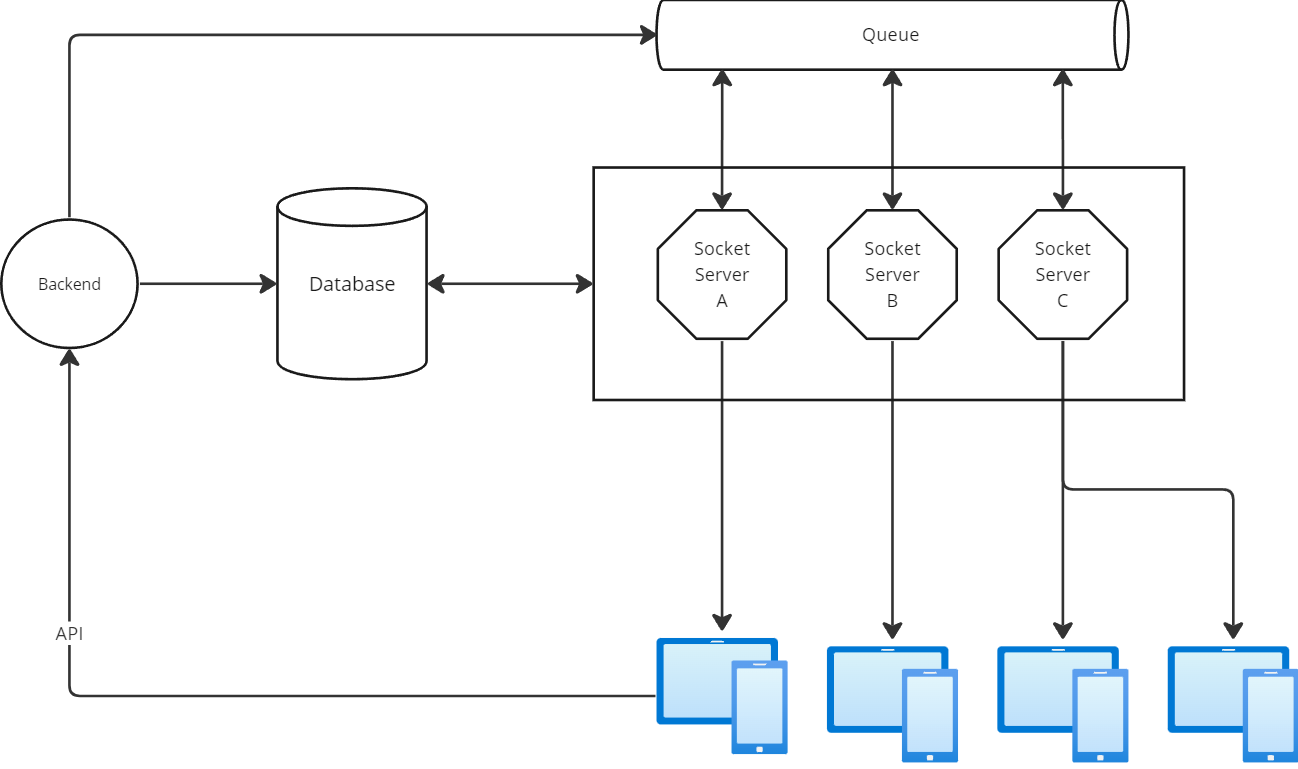
\includegraphics[width=\textwidth]{images/hChip/RabbitMQ/notification-design.png}
	\caption{Kiến trúc tổng quan của hệ thống thông báo}
	\label{fig:notification-design}
\end{figure}

Socket.IO là một thư viện JavaScript cho phép giao tiếp theo thời gian thực, hai chiều trên máy chủ và máy khách bằng cách thiết lập một kênh truyền dữ liệu (kết nối socket) giữa máy chủ và máy khách, cho phép truyền dữ liệu theo cả hai hướng.
Áp dụng quy tắc đó ở các hệ thống lớn với kiến trúc vi dịch vụ, các vi dịch vụ sẽ mở các kết nối socket với nhau nhằm tạo ra một kênh liên lạc giúp thông báo các sự kiện từ phía người dùng đến các vi dịch vụ khác để xử lý nó.

Khi sử dụng Socket.IO, kiến trúc của socket sẽ có thêm một adapter đi kèm như trên Hình~\ref{fig:socket-adapter}.
Tuy nhiên đối với mô hình này, khi hệ thống có mở rộng và có nhiều máy chủ hơn, máy chủ được sử dụng làm adpter (ở đây là Redis) sẽ cần phải liên tục gửi yêu cầu đến tất cả các adapter còn lại mỗi khi một máy chủ gửi thông tin đến do máy chủ gửi tin không hề biết là máy khách cần nhận tin đang kết nối tới máy chủ nào.
Điều này dẫn đến giảm tải hiệu năng của đáng kể khi mở rộng hệ thống do các kết nối không cần thiết giữa các máy chủ với nhau.

\begin{figure}[ht]
	\centering
	
\includegraphics[width=\textwidth]{images/hChip/RabbitMQ/socket-adapter.png}
	\caption{Kiến trúc của socket adapter ~\protect\footnotemark}
	\label{fig:socket-adapter}
\end{figure}
\footnotetext{https://socket.io/docs/v4/redis-adapter/}

Ngoài ra, cơ chế Publisher/Subscriber (Pub/Sub) giúp gửi và nhận dữ liệu giữa các máy chủ thông qua socket cũng mang một hạn chế đó là máy chủ gửi dữ liệu đi không có cơ chế đảm bảo dữ liệu đến được với máy nhận.

Cho nên để đảm bảo tin nhắn được gửi đến đúng máy khách, thiết kế của hệ thống thông báo đã được thay đổi, tận dụng thêm một cơ sở dữ liệu giúp lưu trữ thông tin của các máy chủ và máy khách kết nối với nhau.
Điều này giúp tránh việc phải gọi đến mọi máy sub khi một máy gửi tin nhắn lên do cơ sở dữ liệu lưu trữ mọi hoạt động kết nối và ngắt kết nối giữa máy khách và các máy chủ socket.
Thiết kế chi tiết về cơ sở dữ liệu của hệ thống quản lý tin nhắn áp dụng với hệ thống thông báo của nền tảng quản lý quán ăn sẽ được đề cập trong Mục~\nameref{sec:database-design}.

Ngoài ra trong Hình~\ref{fig:notification-design}, hệ thống cũng sử dụng một hàng đợi, ở đây là RabbitMQ nhằm cân bằng tải tới các máy chủ socket, phân loại và xử lý tin nhắn giúp chuyển tiếp tin nhắn đến đúng máy khách cần nhận tin.
Ngoài ra việc sử dụng hàng đợi tin nhắn (message queue) còn hỗ trợ lưu trữ tin nhắn khi máy khách ngắt kết nối khỏi hệ thống thông báo và đợi cho đến khi máy khách kết nối trở lại nhằm thực hiện lại tác vụ.

\section{Cấu trúc cơ sở dữ liệu} \label{sec:database-design}
Tại bất kỳ dự án phát triển phần mềm nào, có một giai đoạn đóng vai trò không thể thiếu đó là thiết kế cơ sở dữ liệu.
Việc thiết kế cơ sở dữ liệu sẽ bắt dầu trước mọi quá trình xây dựng sản phẩm, giai đoạn này sẽ đi cùng với giai đoạn thiết kế các màn hình, các ca sử dụng của hệ thống.
Đối với nền tảng quản lý quán ăn, tổng cộng có bốn cơ sở dữ liệu trong đó đối mỗi cơ sở dữ liệu sẽ đảm nhiệm vai trò lưu trữ cho từng vi dịch vụ trong hệ thống.
Mỗi cơ sở dữ liệu sẽ có các trường được thiết kế đảm bảo việc lưu trữ các trường thông tin phục vụ cho luồng nghiệp vụ.
\subsection{Dịch vụ quản lý cửa hàng}
Cơ sở dữ liệu của dịch vụ quản lý cửa hàng được thiết kế với mục đích quản lý thông tin về sản phẩm, các loại dịch vụ và hoạt động chung của nhà hàng, quán ăn vừa và nhỏ.
Trong đó, các trường thông tin được tổ chức thành các bảng chính như Hình~\ref{fig:product-service-database-design}.

\begin{figure}[ht]
	\centering
	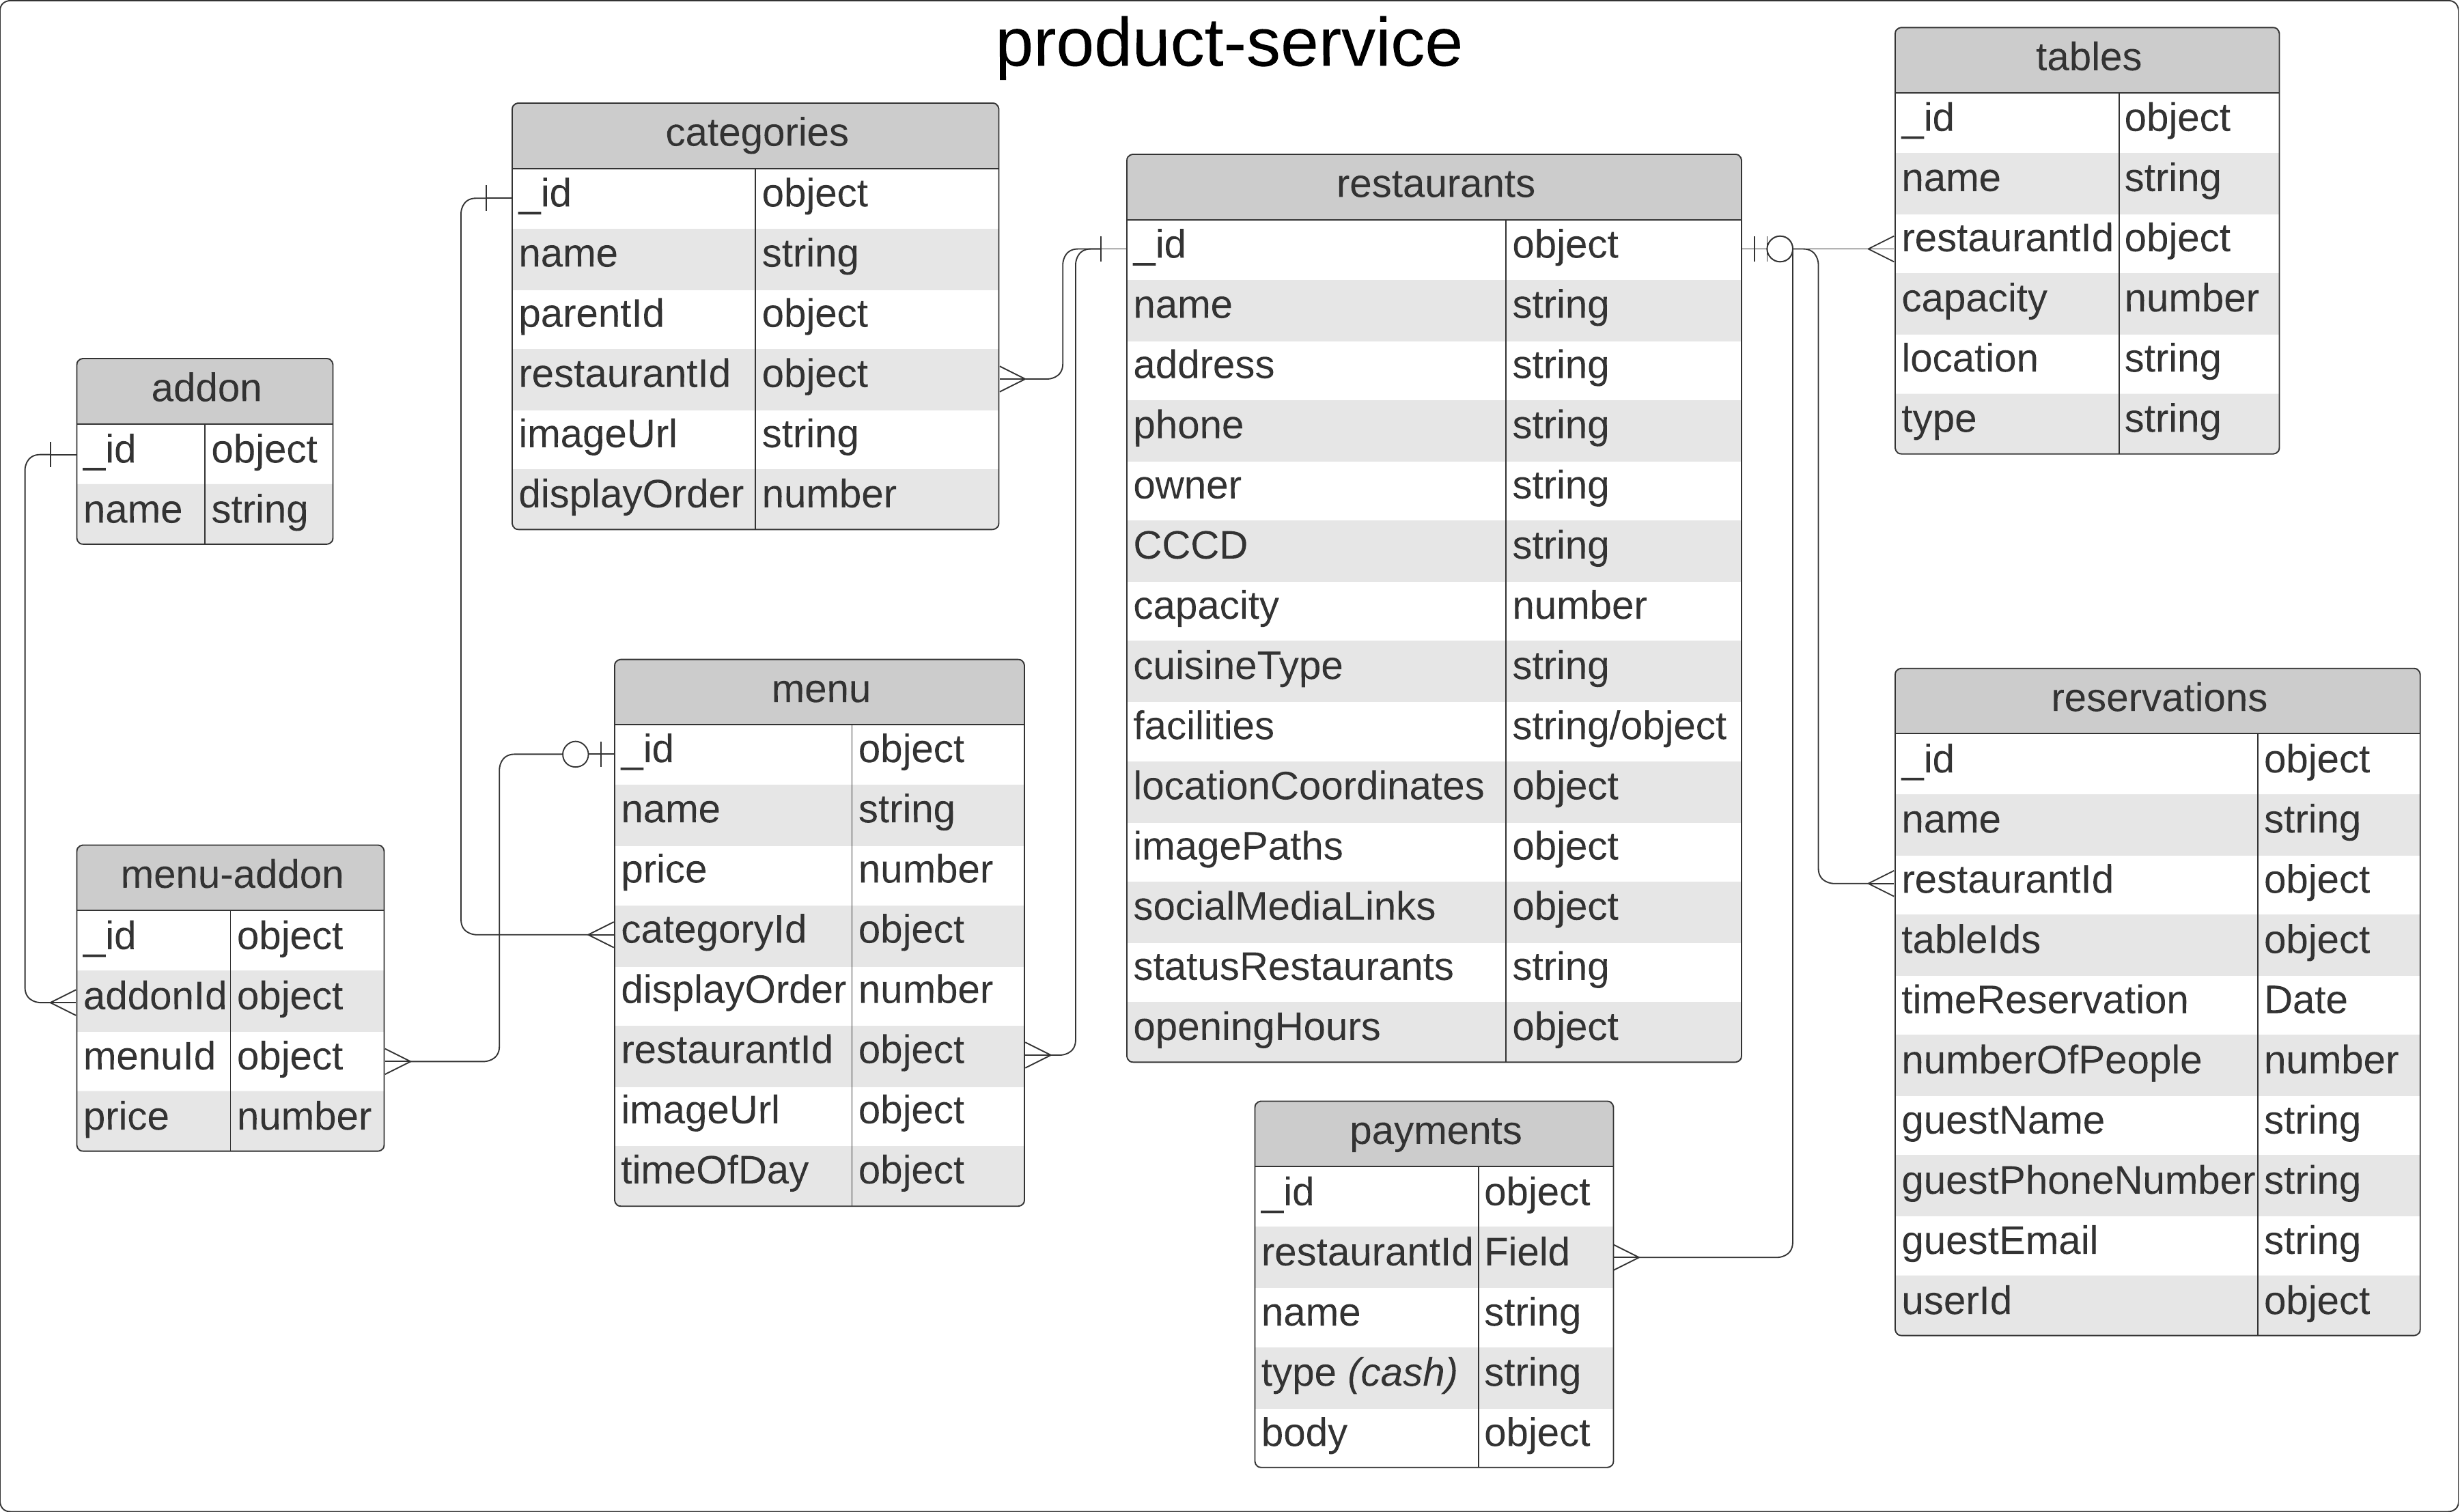
\includegraphics[width=\textwidth]{images/hChip/MongoDB/product-service-design.png}
	\caption{Thiết kế cơ sở dữ liệu cho dịch vụ quản lý cửa hàng}
	\label{fig:product-service-database-design}
\end{figure}

Các bảng tại Hình~\ref{fig:product-service-database-design} bao gồm bảng \tcode{restaurants} lưu thông tin của nhà hàng như tên, địa chỉ, số điện thoại, thông tin liên hệ của chủ sở hữu, v.v. giúp khách hàng có thể dễ dàng tìm kiếm, liên hệ khi cần đặt bàn, trợ giúp.
Tại đây, một nhà hàng sẽ bao gồm nhiều thông tin khác như thông tin về đặt bàn được lưu trữ ở bảng \tcode{reservations} bao gồm tên khách hàng, số điện thoại, thời gian đặt bàn, v.v., thông tin về các bàn của quán ăn nằm ở bảng \tcode{tables} lưu sức chứa và vị trí của bàn.
Thực đơn của quán ăn sẽ được lưu trong một tập hợp các bảng bao gồm bảng \tcode{menu} lưu các thông tin như tên, giá, loại món ăn cũng như là thời gian bán của món trong ngày.
Mỗi món sẽ được phân loại vào một bảng \tcode{categories}, bảng này bao gồm trường \tcode{parentId} hỗ trợ lồng các thể loại món với nhau giúp dễ dàng quản lý.
Cuối cùng, bảng \tcode{payments} lưu trữ thông tin về các phương thức thanh toán nhà hàng hỗ trợ như tiền mặt, chuyển khoản, v.v.

\subsection{Dịch vụ quản lý định danh khách hàng}
Cơ sở dữ liệu \tcode{id-service} được thiết kế nhằm quản lý thông tin của người dùng trong hệ thống và các mối quan hệ liên quan đến nhà hàng.
Hình~\ref{fig:id-service-database-design} mô tả kiến trúc cơ sở dữ liệu mô hình quản lý định danh khách hàng bao gồm bảng \tcode{user} lưu các thông tin cơ bản về người dùng bao gồm tên, tuổi, số điện thoại, địa chỉ, v.v.
Ngoài thông tin của người dùng còn có các bảng lưu danh sách các nhà hàng người dùng đã từng đến ăn, nhà hàng người dùng đang theo dõi và các nhà hàng mà người dùng thích.
Các trường thông tin tại bảng \tcode{users} được người dùng điền khi chỉnh sửa thông tin hồ sơ của bản thân hoặc trong trường hợp người dùng đăng nhập thông qua một bên thứ ba như Google, Facebook, hệ thống sẽ truy cập các thông tin công khai của người dùng trên nền tảng đó.
\begin{figure}[H]
	\centering
	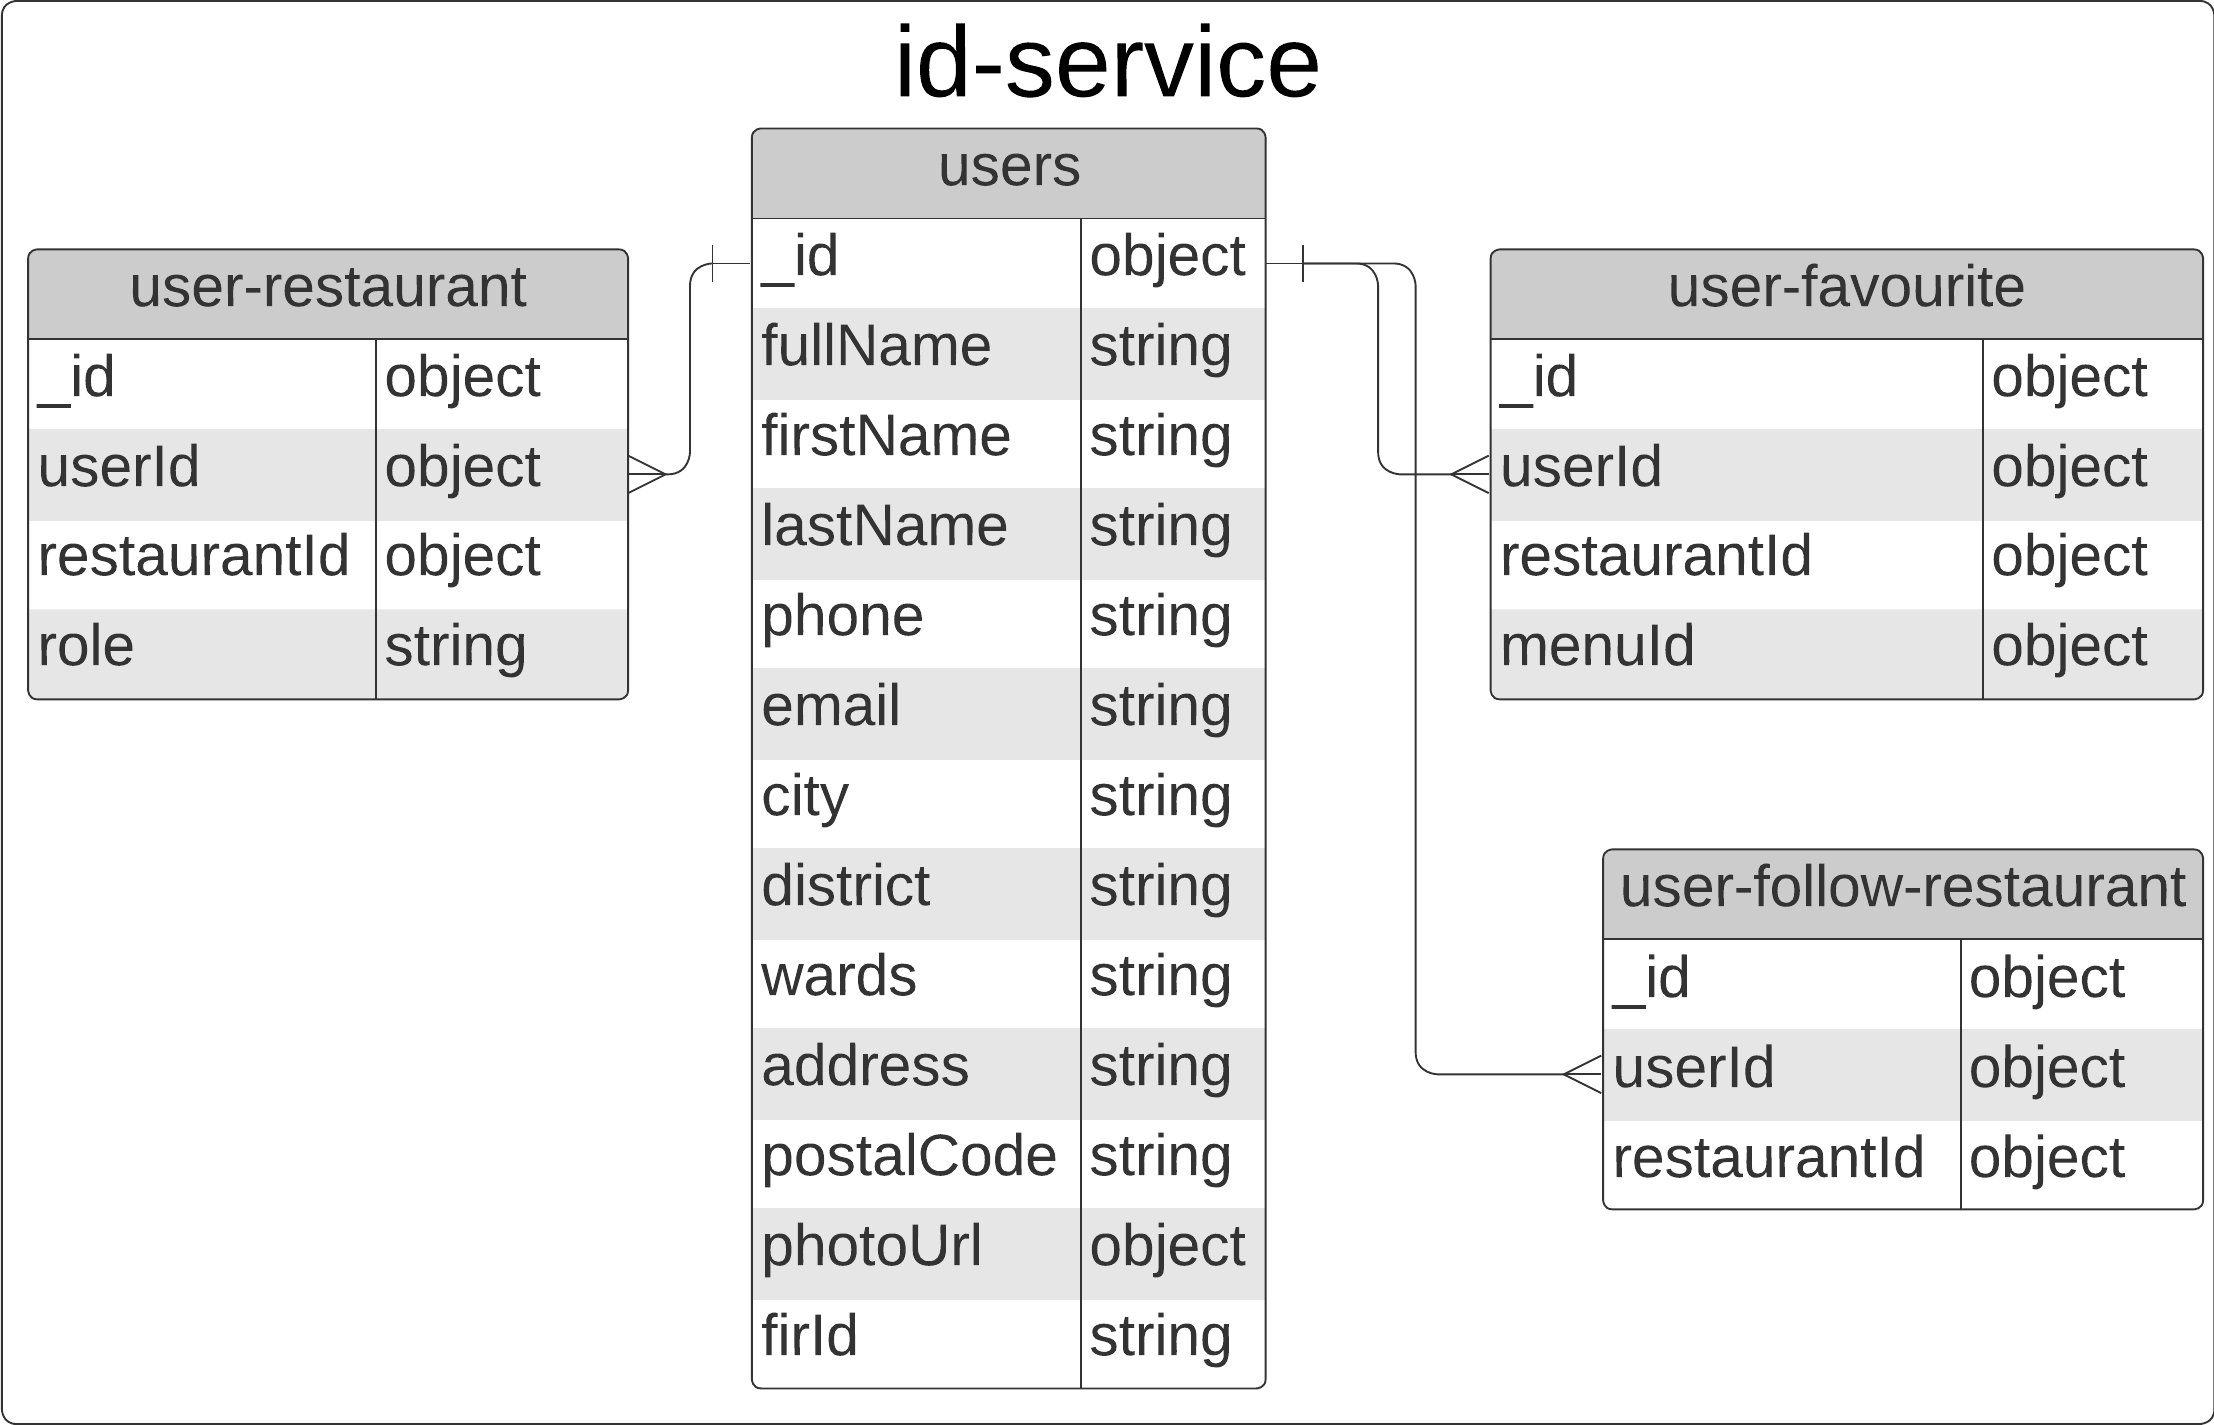
\includegraphics[width=\textwidth]{images/hChip/MongoDB/id-service-design.png}
	\caption{Thiết kế cơ sở dữ liệu cho dịch vụ quản lý định danh khách hàng}
	\label{fig:id-service-database-design}
\end{figure}

\subsection{Dịch vụ thông báo}
Mục đích của cơ sở dữ liệu \tcode{notification-service} là quản lý các thông báo, lời gọi giữa các dịch vụ với nhau thông qua socket trong hệ thống.
Cơ sở dữ liệu này bao gồm 2 bảng là \tcode{socket-history} và \tcode{messages}.
Trên Hình~\ref{fig:notification-service-database-design}, bảng \tcode{socket-history} lưu trữ lịch sử kết nối socket, bao gồm thông tin về khách hàng \tcode{ownerId}, \tcode{socketId} lưu trữ thông tin của phiên kết nối đó, và các trường lưu thông tin của máy chủ cũng như trạng thái, thời gian máy khách kết nối, ngắt kết nối khỏi hệ thống.
\begin{figure}[H]
	\centering
	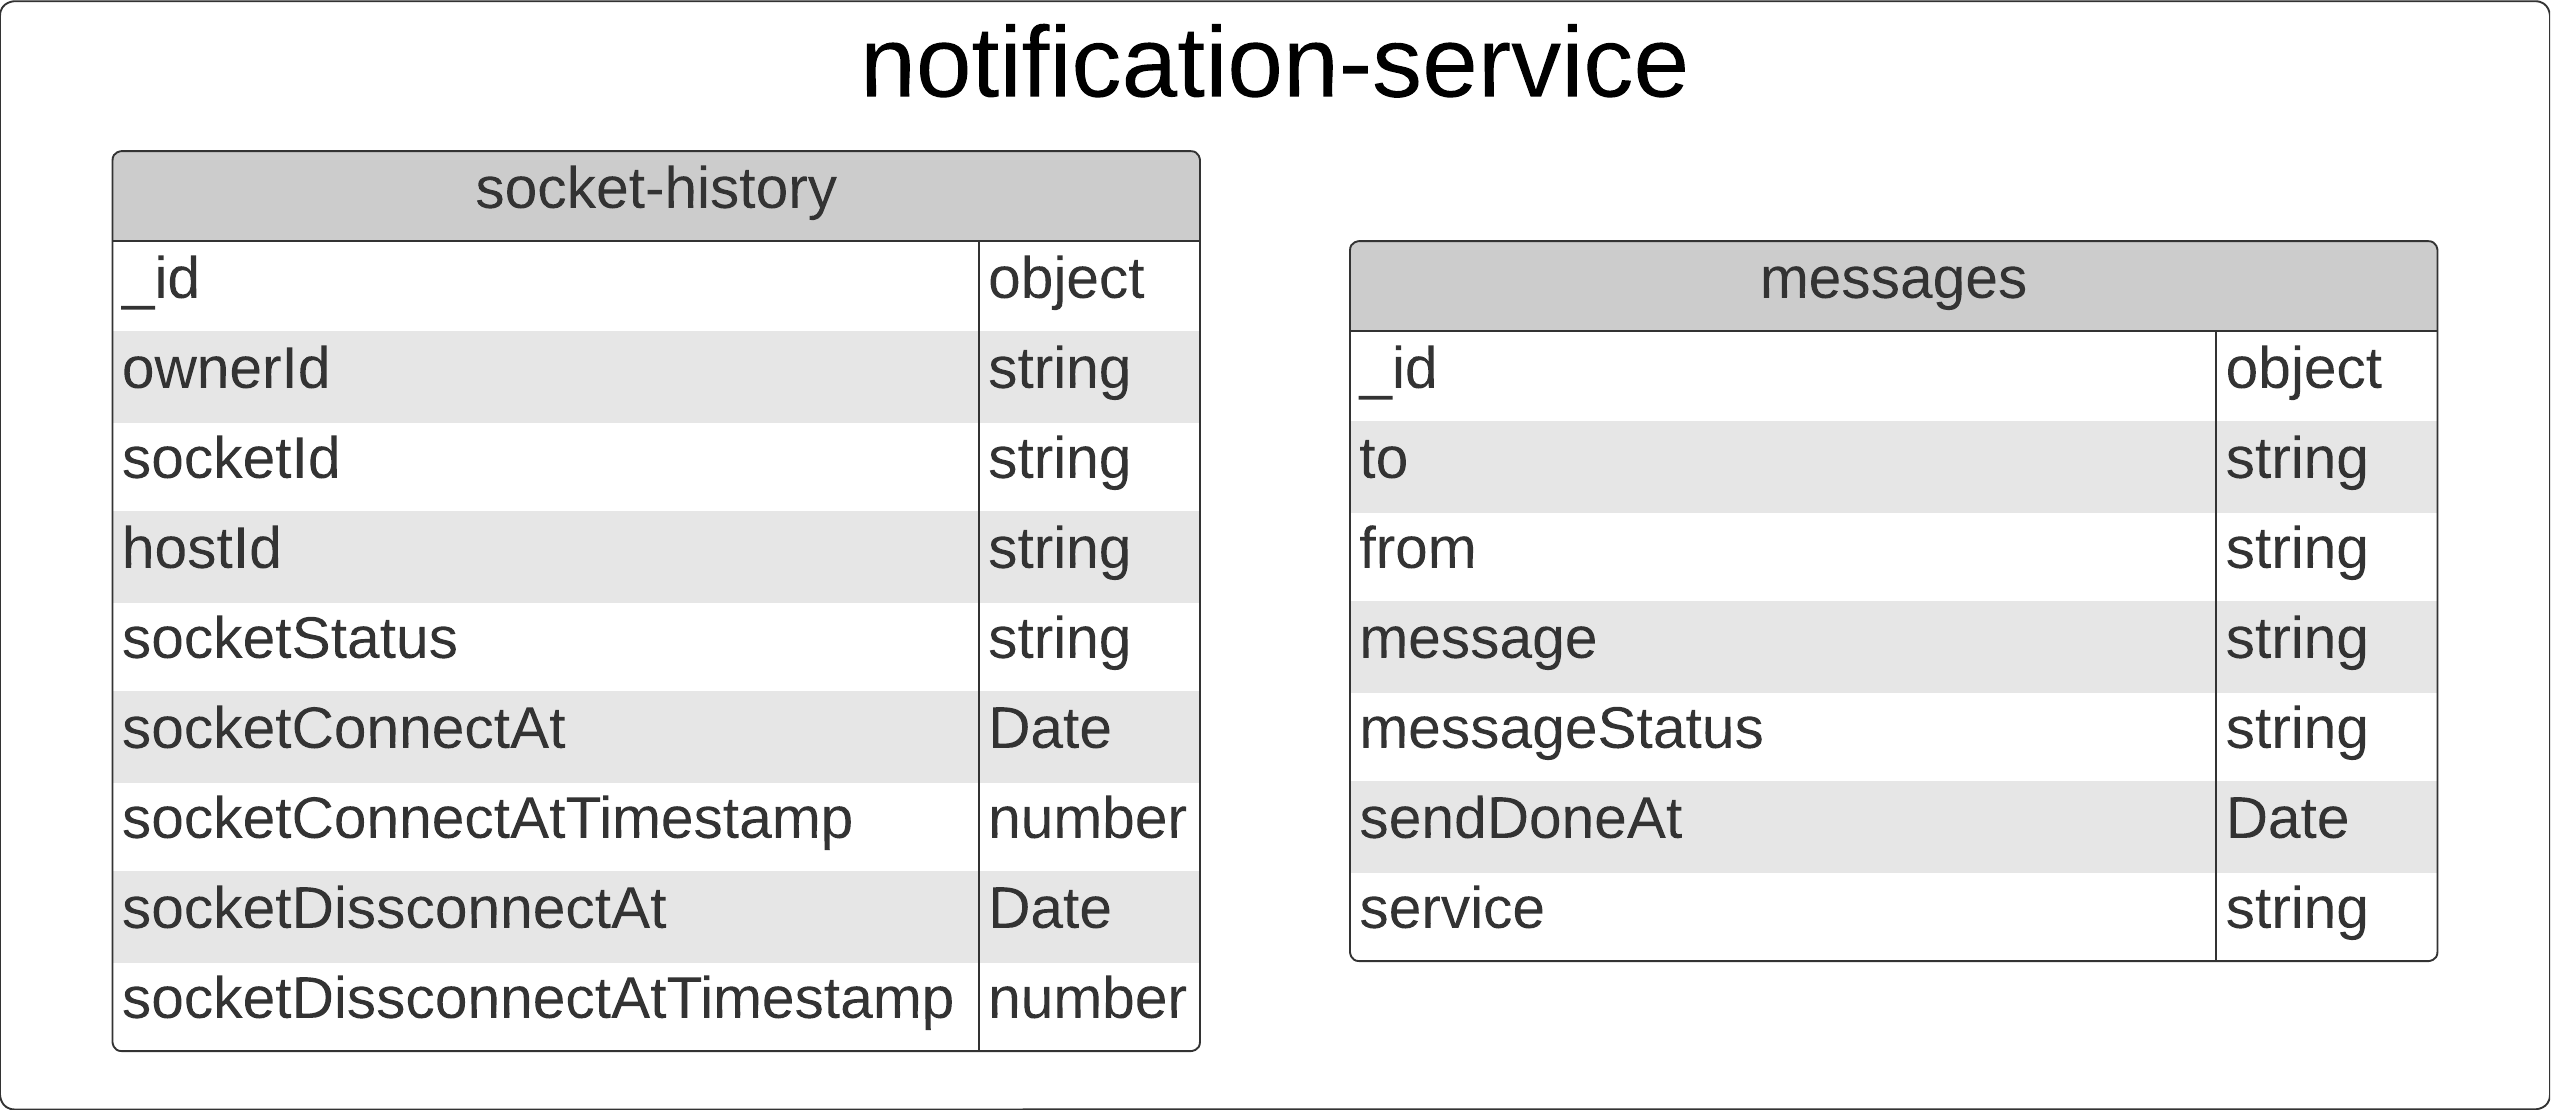
\includegraphics[width=\textwidth]{images/hChip/MongoDB/notification-service-design.png}
	\caption{Thiết kế cơ sở dữ liệu cho dịch vụ thông báo}
	\label{fig:notification-service-database-design}
\end{figure}

\subsection{Dịch vụ đặt bàn}
Cơ sở dữ liệu \tcode{order-service} quản lý các khía cạnh trong quy trình đặt món và thanh toán trong hệ thống quản lý nhà hàng.
Cơ sở dữ liệu cũng được thiết kế với cơ chế đánh giá giúp khách hàng có thể nêu lên ý kiến của họ với nhà hàng giúp nhà hàng nắm được cảm nhận của khách.
Hình~\ref{fig:order-service-database-design} bắt đầu từ bảng \tcode{orders} ở giữa lưu trữ thông tin tổng quan về mỗi đơn hàng bao gồm \tcode{customerId} (Id của khách hàng), \tcode{restaurantId} (Id nhà hàng), \tcode{tableId} (Id bàn ăn), người phục vụ của bàn \tcode{staffId} và thời gian cũng như trạng thái của đơn hàng.
Bảng \tcode{order-details} đi sâu vào chi tiết từng món ăn trong mỗi đơn hàng bao gồm Id của món \tcode{menuId}, số lượng và tổng giá tiền cũng như là các tùy chọn khác tại trường \tcode{specialRequests}
Để quản lý thông tin hóa đơn cho mỗi đơn hàng, bảng \tcode{invoices} sẽ lưu thông tin về giá trị đơn hàng, phí dịch vụ, thuế cũng như là người phụ trách thanh toán cho đơn hàng đó.
\begin{figure}[H]
	\centering
	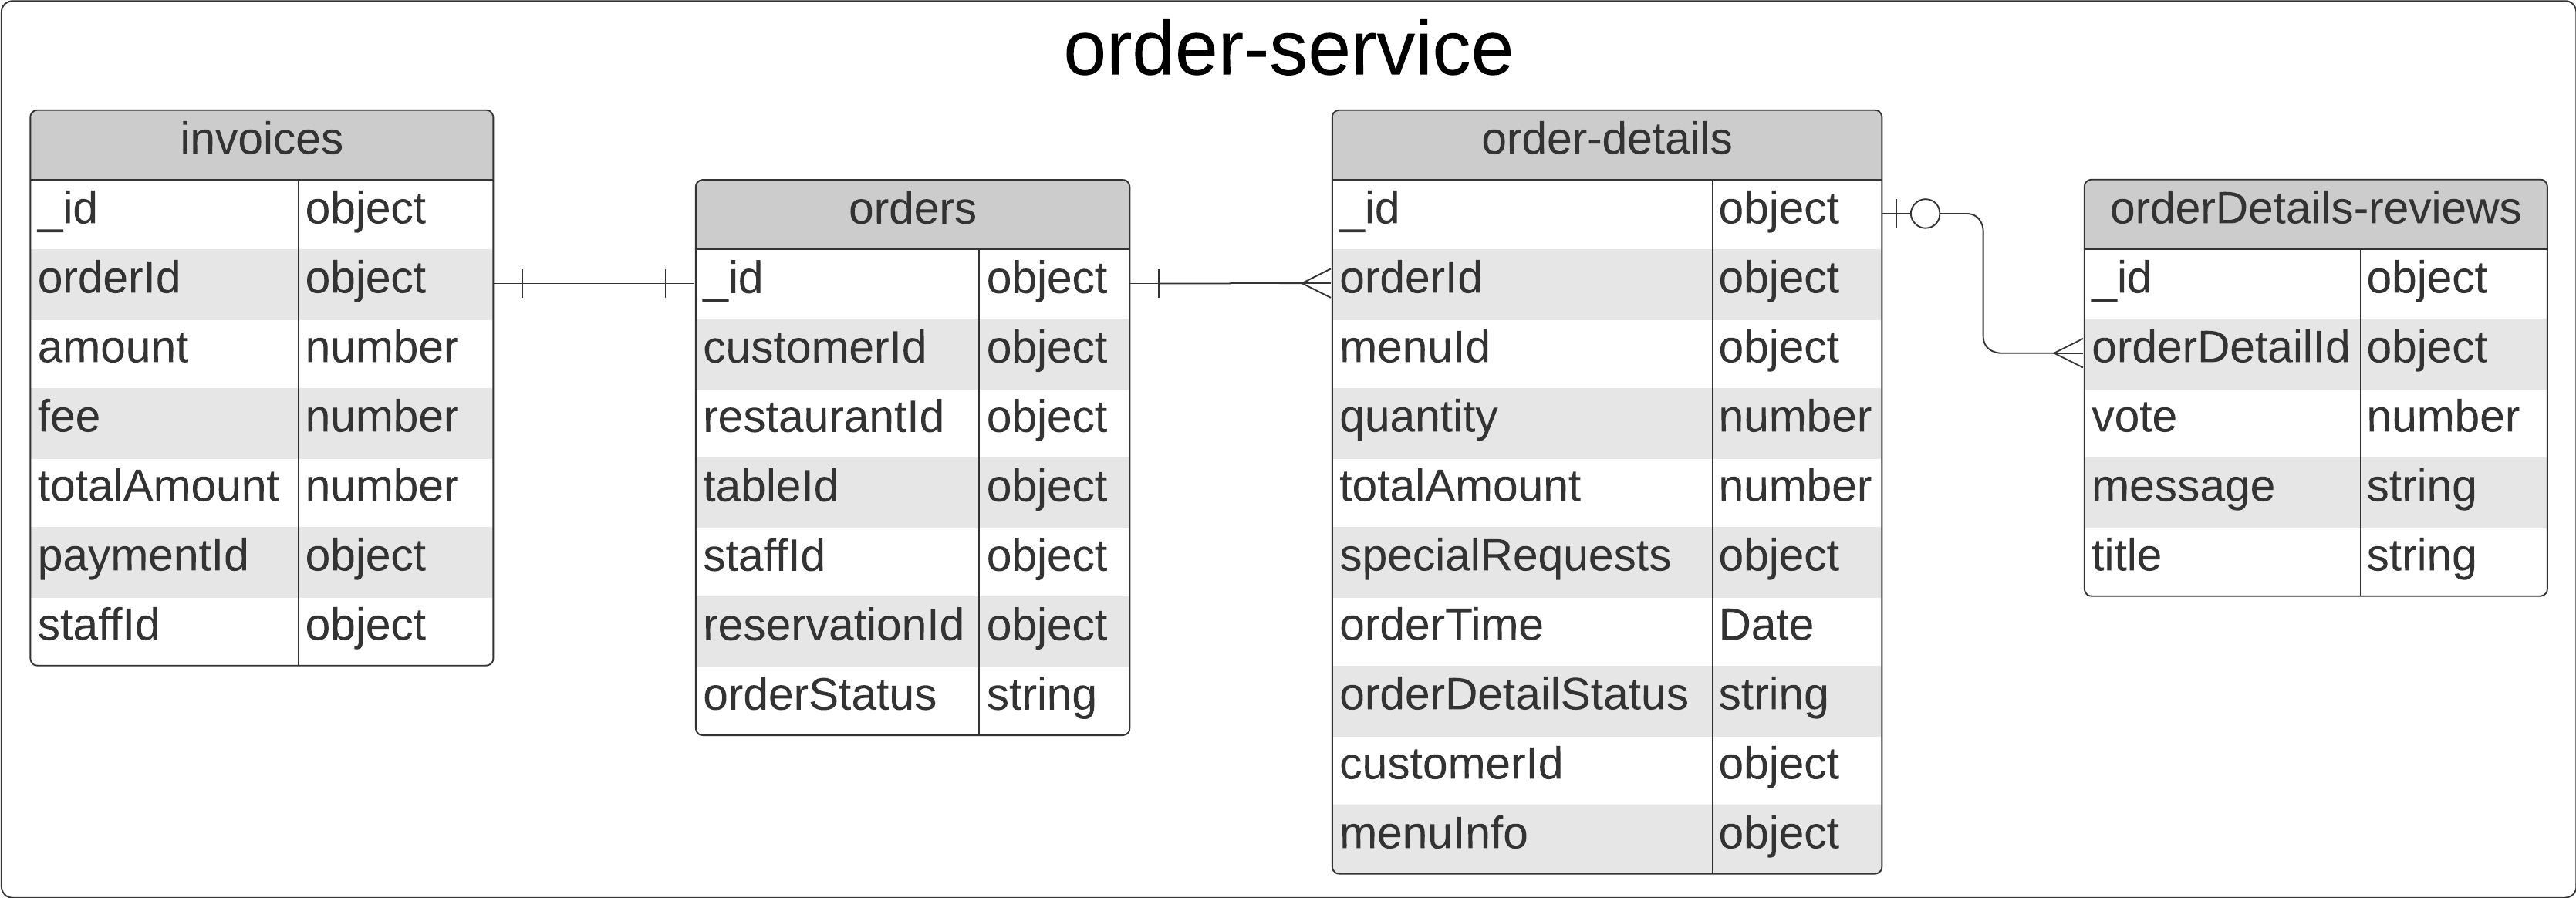
\includegraphics[width=\textwidth]{images/hChip/MongoDB/order-service-design.png}
	\caption{Thiết kế cơ sở dữ liệu cho dịch vụ đặt bàn}
	\label{fig:order-service-database-design}
\end{figure}

\section{Luồng người dùng}\label{sec:user-journey}
Thiết kế luồng người dùng (use journey) là một quá trình trực quan hóa quan giúp đội ngũ phát triển hiểu rõ hành vi, nhu cầu của người dùng khi tương tác với giao diện sản phẩm hệ thống.
Việc xây dựng luồng người dùng đầy đủ và chi tiết cho phép người xem có cái nhìn toàn diện, đẩy đủ nhất về trải nghiệm của người dùng (UX) từ lúc bắt đầu tương tác với hệ thống cho đến khi hoàn thành chức năng đề ra, từ đó đưa giúp nhà phát triển ra quyết định điều chỉnh thiết kế phù hợp và tối ưu hóa trải nghiệm người dùng.
Luồng người dùng thường được thể hiện dưới dạng sơ đồ, mô tả các bước mà người dùng thực hiện, các hành động của họ trong từng giai đoạn.
Đối với hệ thống quản lý quán ăn, sẽ có ba giao diện chính đó là giao diện trang giới thiệu hệ thống \tcode{landing-page}, trang quản lý nhà hàng \tcode{admin-page} và trang giao diện cho cửa hàng \tcode{customer-page}.
Trang \tcode{customer-page} sẽ không được mô tả luồng người dùng trong Mục này do nhu cầu tính năng và giao diện của giao diện cửa hàng có thể tùy biến theo yêu cầu của nhà hàng, quán ăn khi họ sử dụng dịch vụ của nền tảng.
\subsection{Trang giới thiệu}
Luồng người dùng trên trang giới thiệu của hệ thống quản lý nhà hàng đi theo hai hướng chính đó là đặt bàn và gia nhập hệ thống với tư cách nhà hàng.
Với tính năng đặt bàn, người dùng truy cập trang giới thiệu, nơi hiển thị danh sách các quán ăn, nhà hàng đã gia nhập nền tảng.
Họ có thể xem danh sách quán, lựa chọn một quán ăn cụ thể để xem thông tin chi tiết cũng như là thực đơn và tiến hành đặt bàn.
Quá trình đặt bàn không yêu cầu người dùng cần phải đăng nhập để thực hiện hành động.

Nếu người dùng quyết định gia nhập hệ thống với tư cách là một chủ nhà hàng, quán ăn, họ sẽ cần phải đăng nhập vào hệ thống.
Sau đó người dùng sẽ truy cập vào trang gia nhập và điền thông tin chi tiết về doanh nghiệp của họ.
Thông tin người dùng nhập sau đó sẽ được xác thực bởi quản trị viên của hệ thống và sẽ liên lạc lại với người đăng ký để xác nhận thủ tục và cấp tài khoản vào hệ thống quản lý nhà hàng.
\begin{figure}[H]
	\centering
	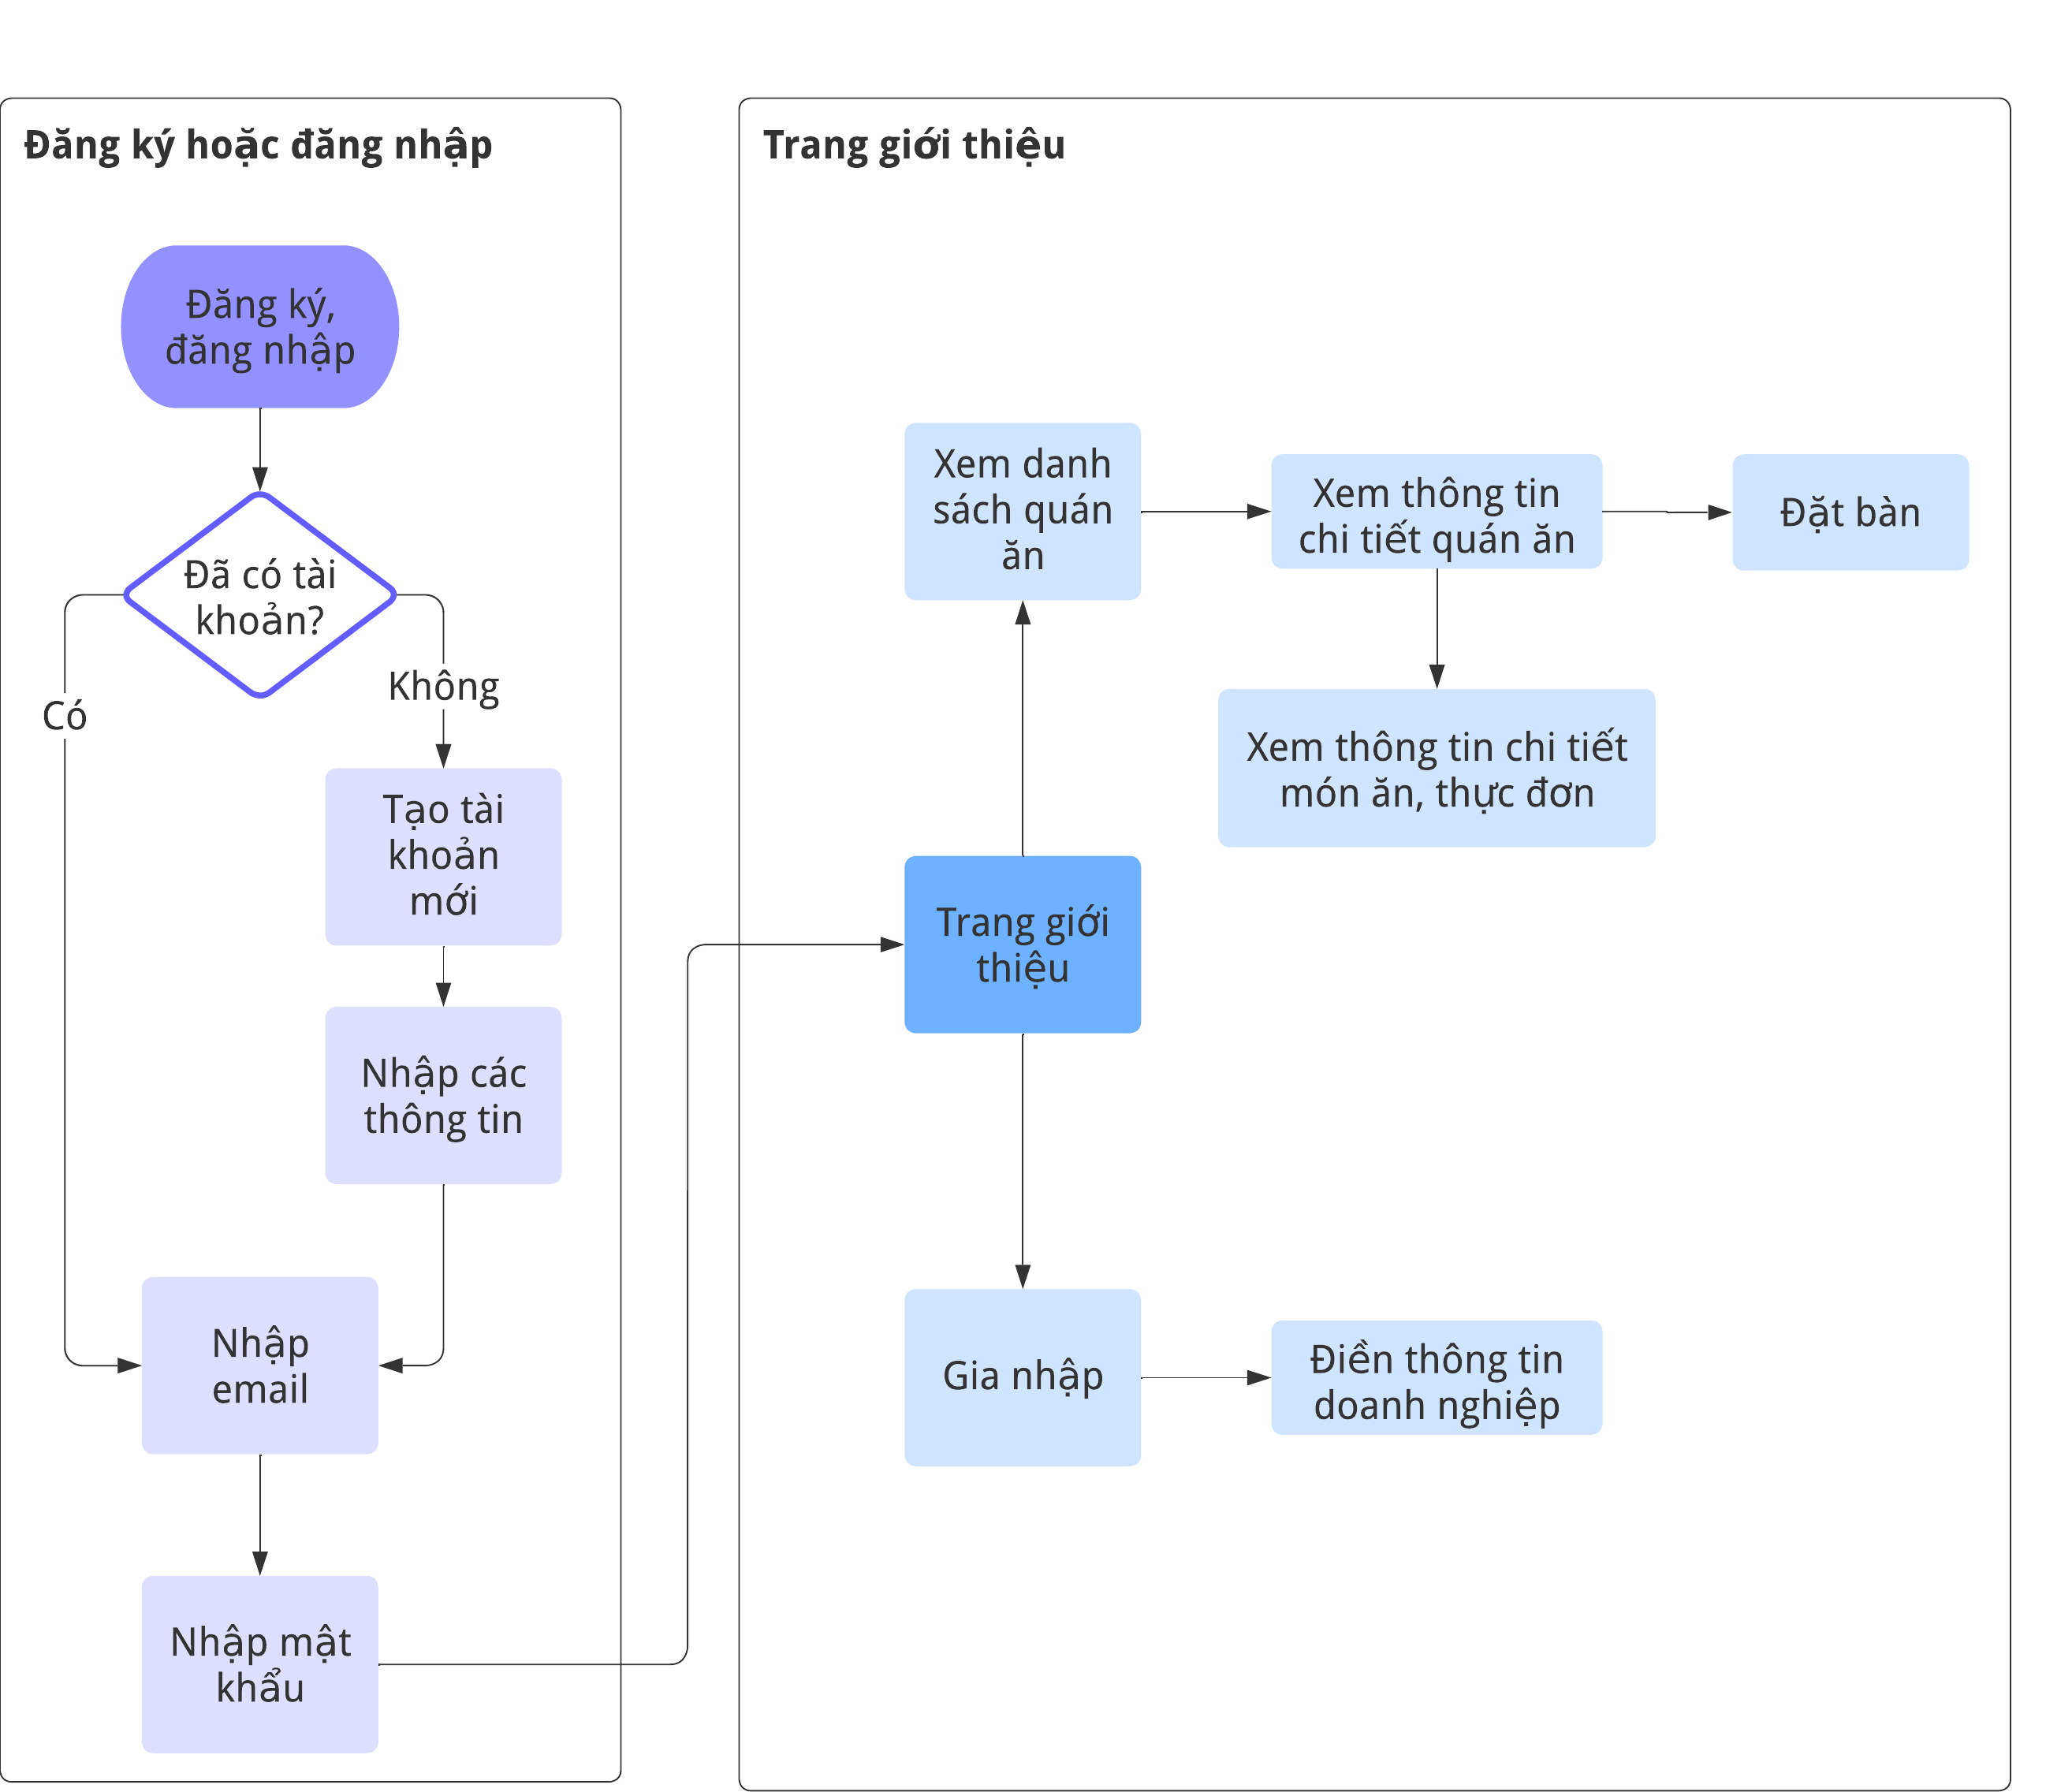
\includegraphics[width=\textwidth]{images/hChip/main-flow/landing-page-user-journey-flow.png}
	\caption{Luồng người dùng trang giới thiệu \tcode{landing-page}}
	\label{fig:landing-page-user-journey}
\end{figure}
\subsection{Quản lý nhà hàng}
Ở trang quản lý nhà hàng, người dùng không thể tự tạo tài khoản mà chỉ có thể đăng nhập dưới các tài khoản được tạo bởi quản trị viên của trang hoặc là quản trị viên hệ thống.
Sau khi đăng nhập vào trang quản lý nhà hàng, các chức năng sẽ được chia ra cho từng vai trò cụ thể.
Nhân viên của nhà hàng, quán ăn được phép xem các thông tin của quán cũng như là thông tin về thực đơn, bàn, đặt bàn, cũng như là thông tin về hóa đơn, doanh thu.
Nhân viên cũng có thể sửa đổi thông tin 
Đối với quản trị viên của trang tức quản lý của cửa hàng, họ có mọi quyền hạn của nhân viên và quản trị viên còn có thể sửa đổi thông tin của nhà hàng, sửa đổi danh sách nhân viên như thêm nhân viên mới, sửa đổi thông tin cá nhân của nhân viên. Ngoài ra quản lý của nhà hàng, quán ăn cũng có thể sửa đổi danh sách các món ăn đang bày bán tại cửa hàng cũng như thay đổi bố cục bàn của quán ăn.
\begin{figure}[H]
	\centering
	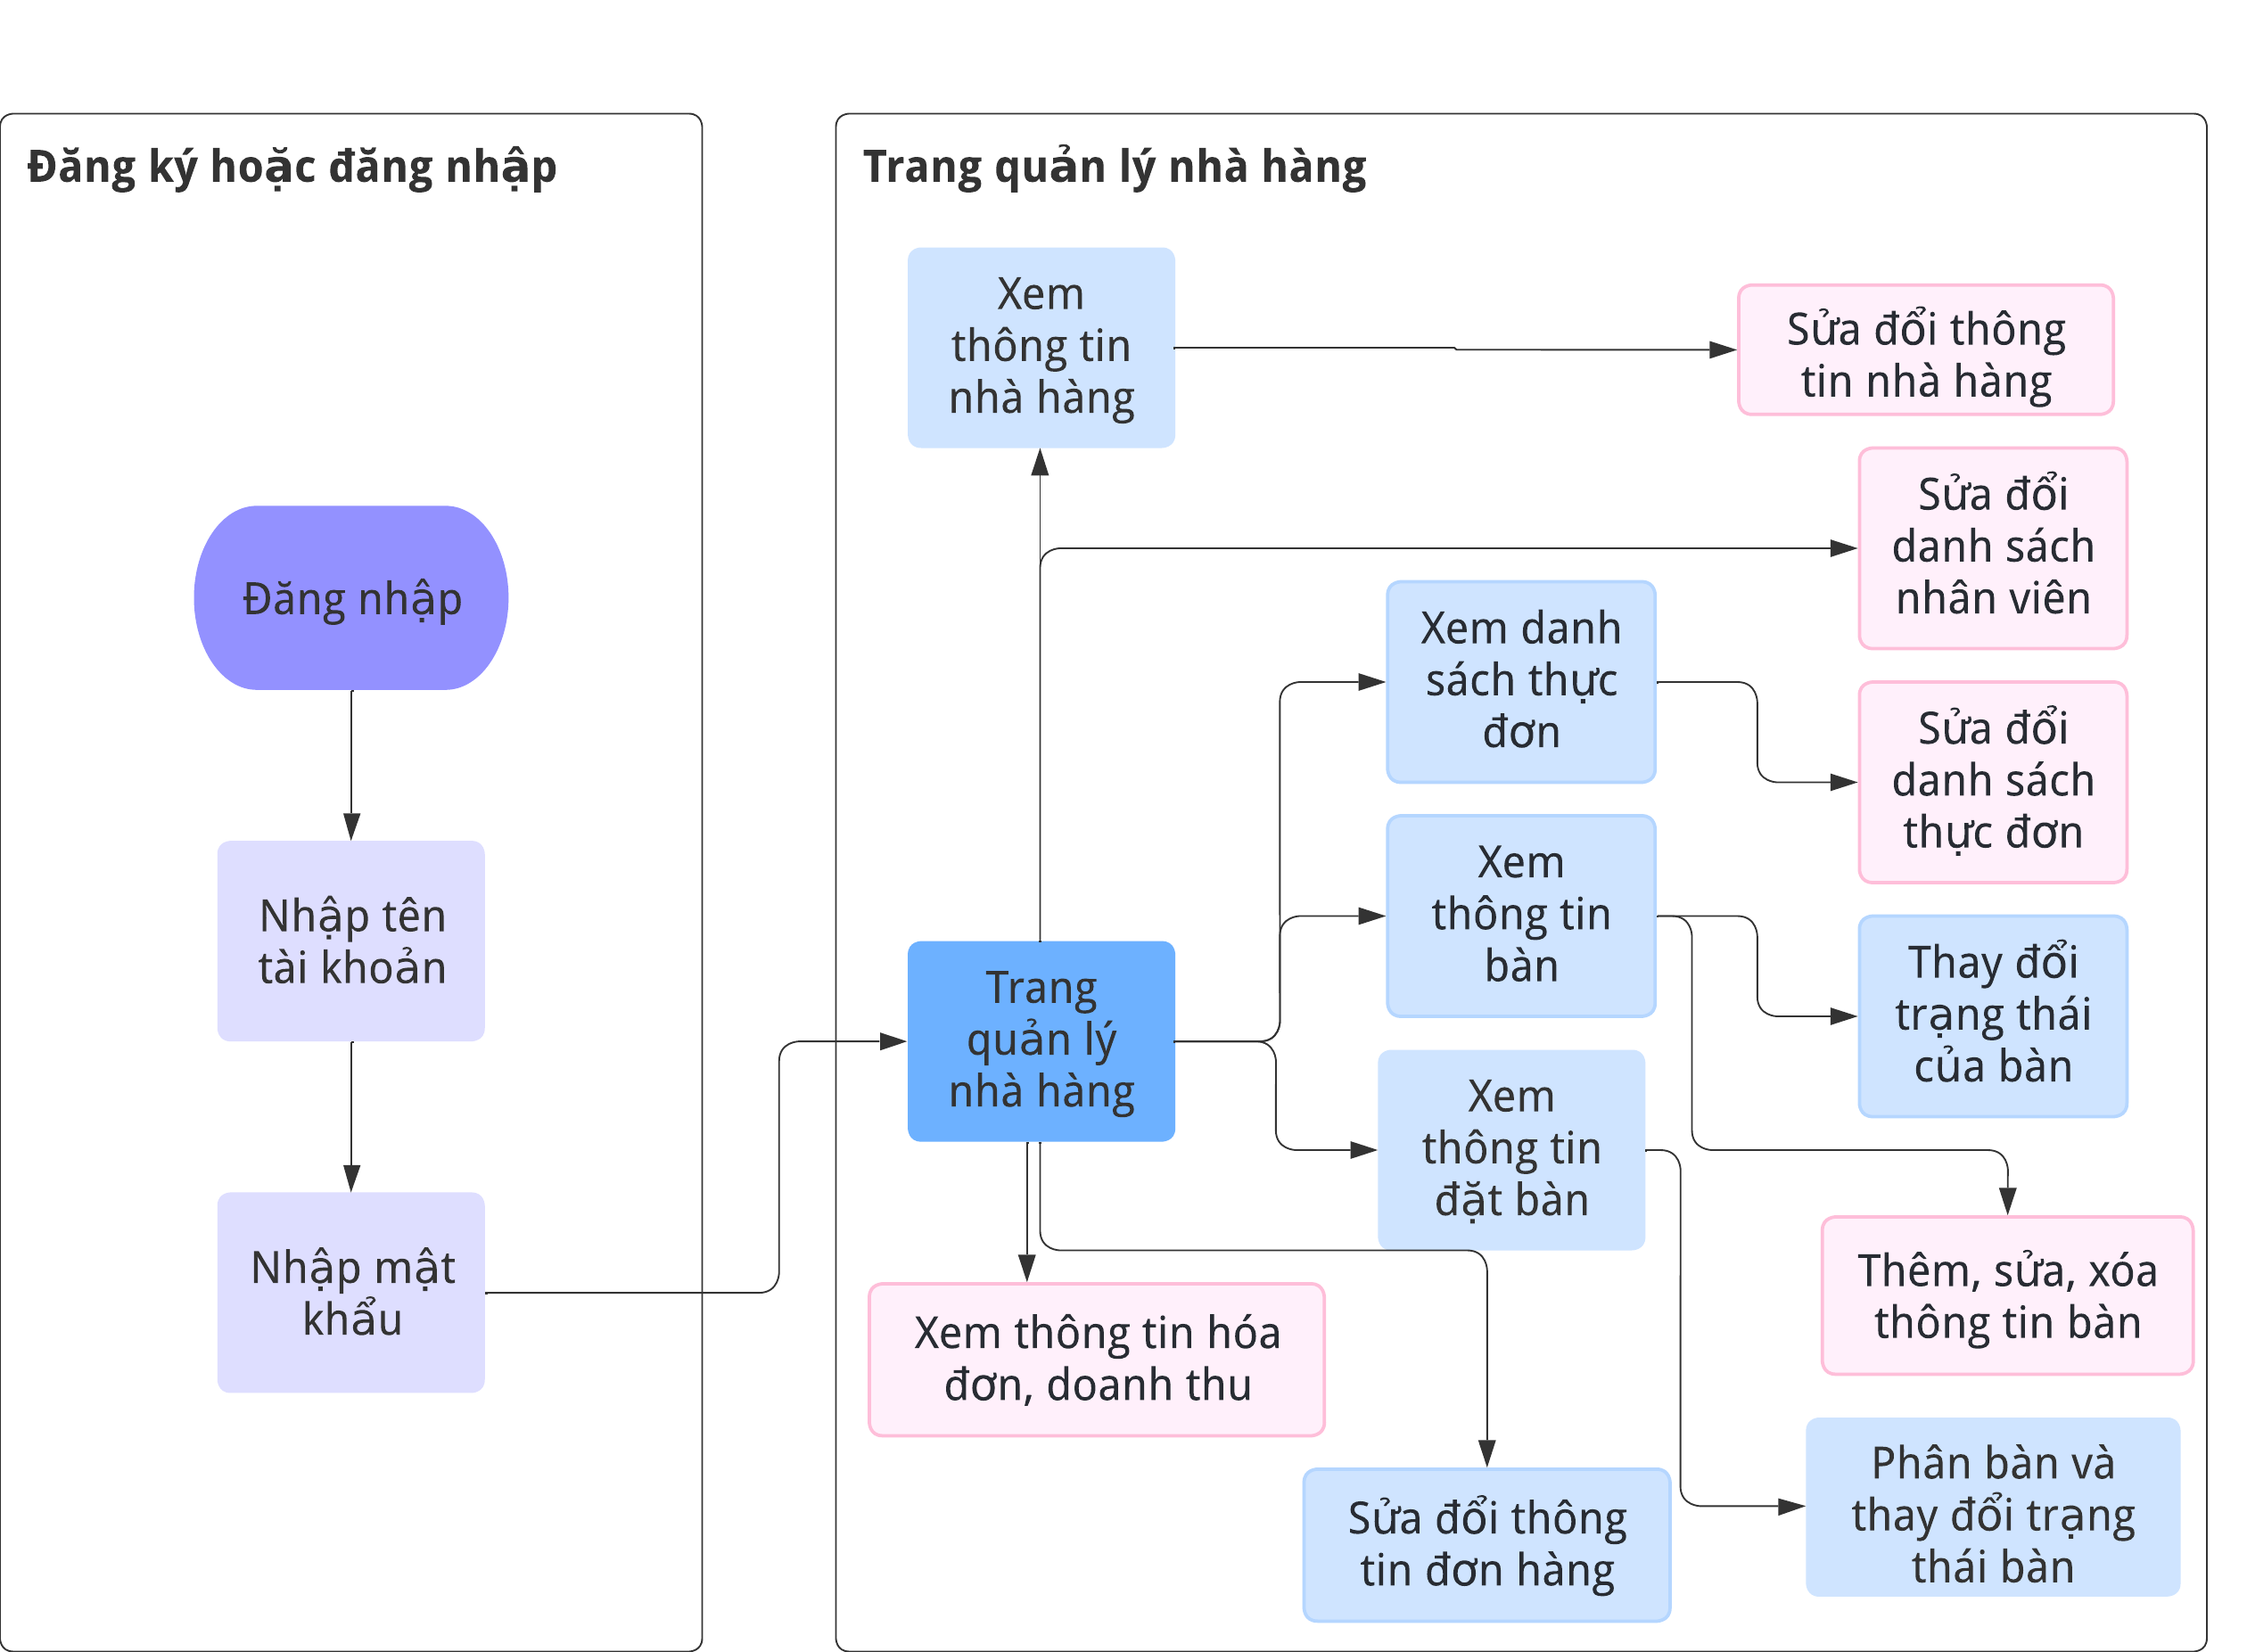
\includegraphics[width=\textwidth]{images/hChip/main-flow/admin-page-user-journey-flow.png}
	\caption{Luồng người dùng trang quản lý quán ăn \tcode{admin-page}}
	\label{fig:admin-page-user-journey}
\end{figure}